

\begin{figure}[th]
	\centering
	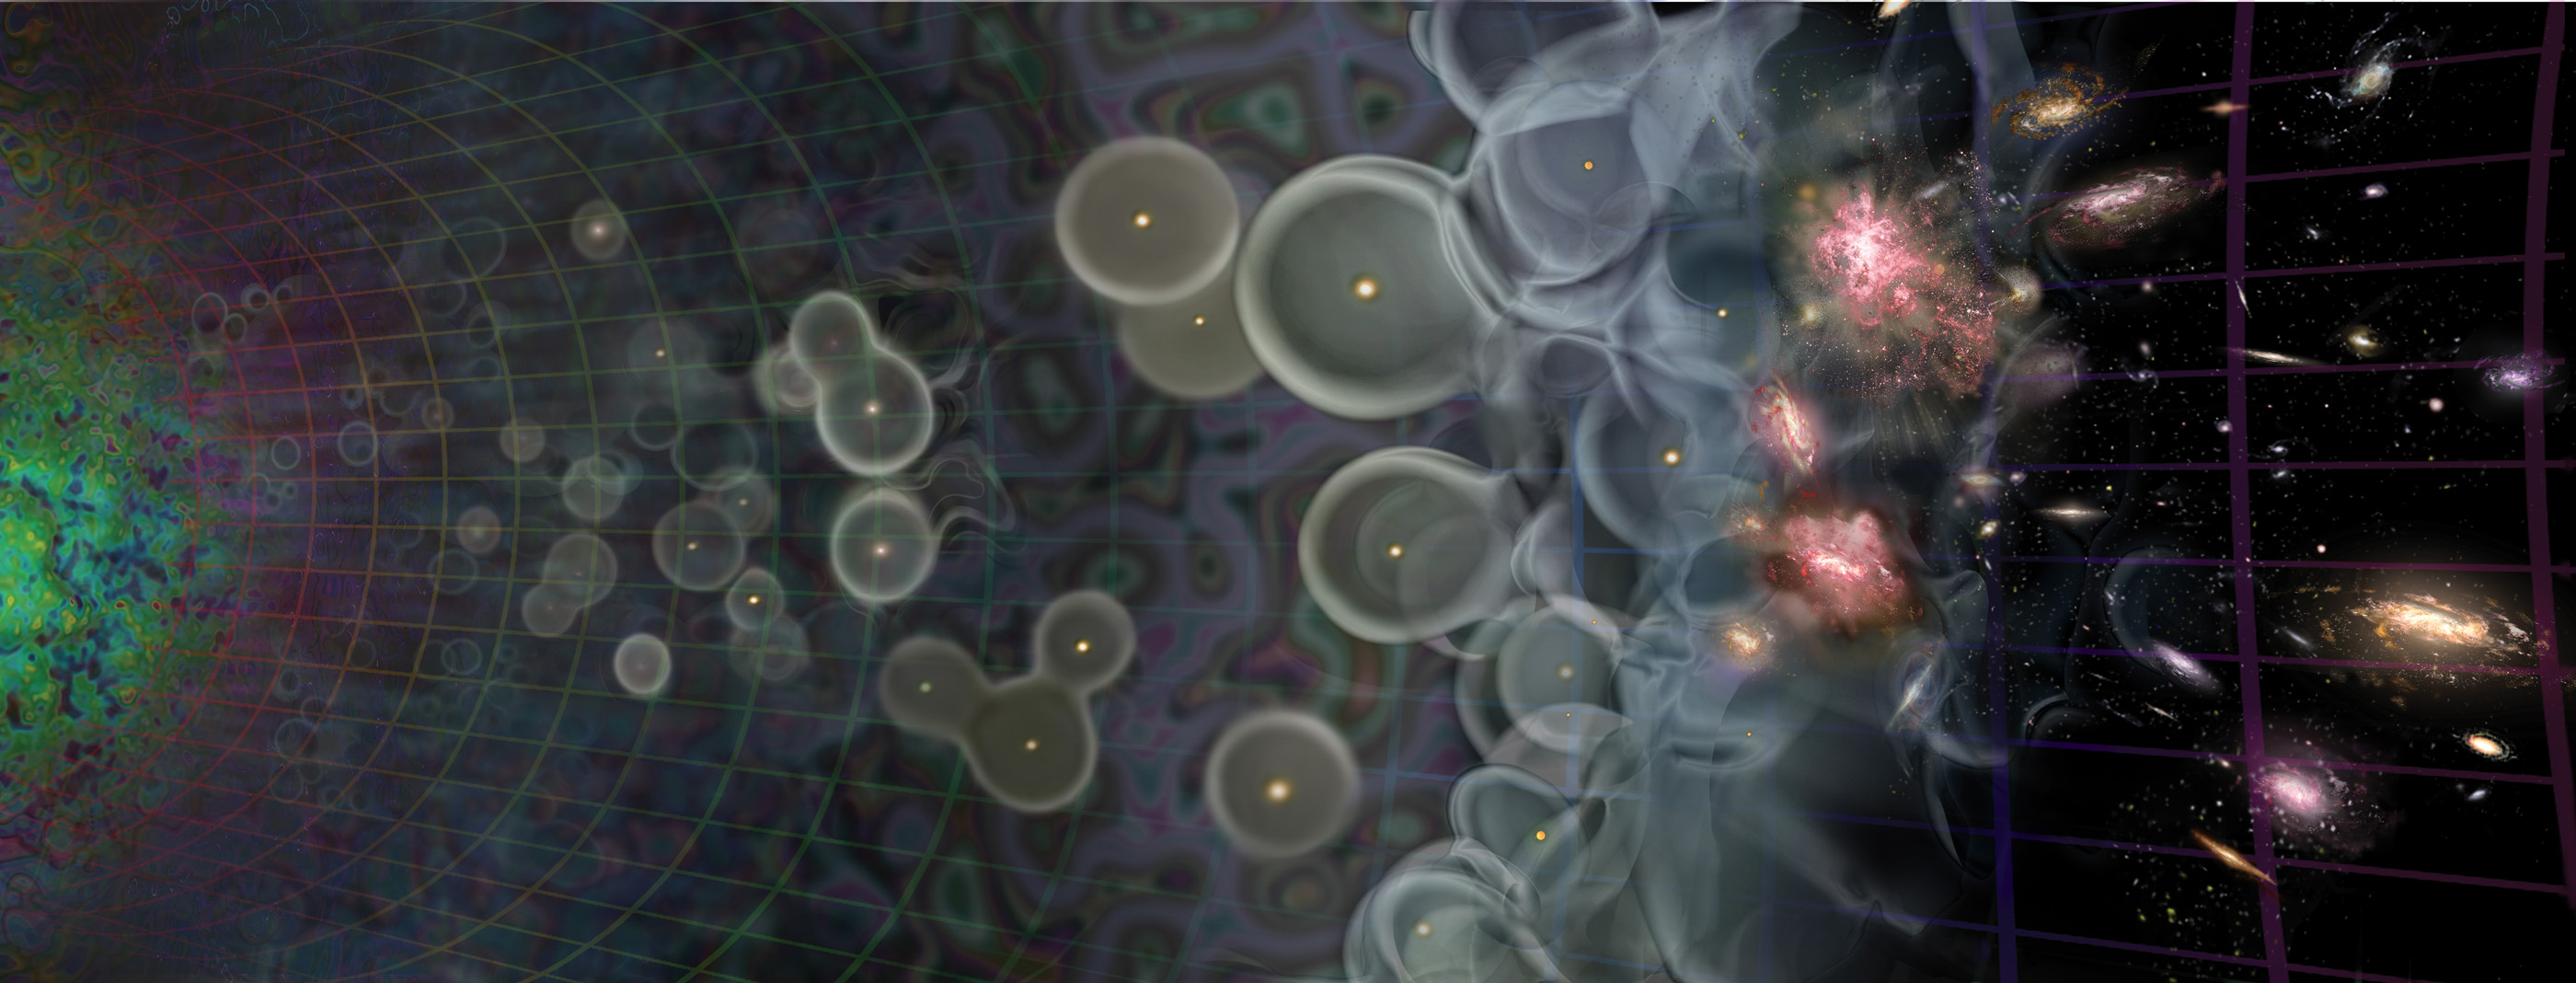
\includegraphics[width=1.0\textwidth]{loeb_sci_american_small.jpg}
	\caption[Epoch of Reionization Timeline]{Timeline of the history of the Universe. To the left, is the CMB. To the right, are the stars and galaxies that exist today.}
	\label{fig:timeline}
\end{figure}

\begin{figure}[th]
	\centering
	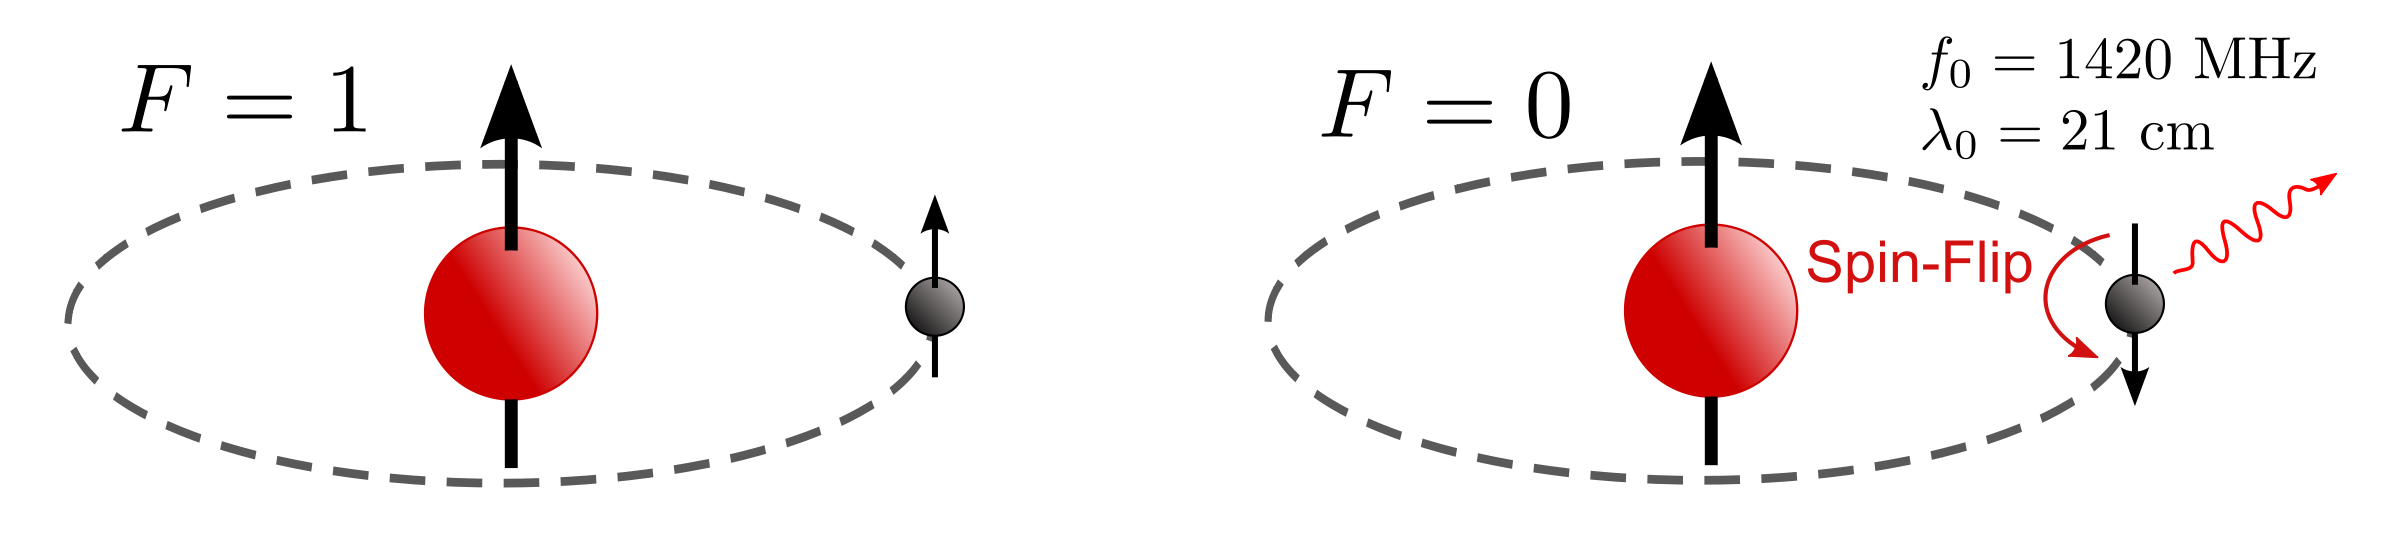
\includegraphics[width=0.90\textwidth]{spin_flip_H.png}
	\caption[Spin-Flip Transition]{A depiction of the spin flip energy transition of neutral hydrogen. Initially,
																					 the spin of the proton and electron are parallel and oriented
																					 in the same direction. The energy transition occurs when the electron's spin spontaneously
																					 flips from the higher energy parallel alignment to the lower energy anti-parallel alignment,
																					 releasing a photon with a wavelength of 21 cm.}
	\label{fig:spin_flip}
\end{figure}
